\documentclass[border=4pt]{standalone}

\usepackage{amsmath}
\usepackage{tikz}
\usepackage{mathdots}
\usepackage{yhmath}
\usepackage{cancel}
\usepackage{color}
\usepackage{siunitx}
\usepackage{array}
\usepackage{multirow}
\usepackage{amssymb}
\usepackage{gensymb}
\usepackage{tabularx}
\usepackage{booktabs}
\usetikzlibrary{fadings}
\usetikzlibrary{patterns}


\begin{document}
 



\tikzset{every picture/.style={line width=0.75pt}} %set default line width to 0.75pt        

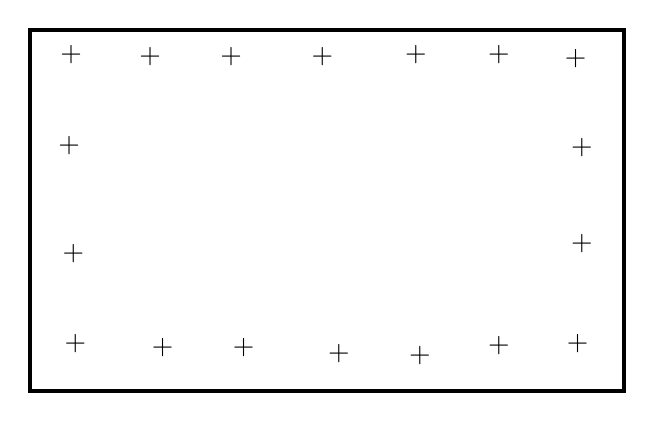
\begin{tikzpicture}[x=0.75pt,y=0.75pt,yscale=-1,xscale=1]
%uncomment if require: \path (0,300); %set diagram left start at 0, and has height of 300

%Shape: Rectangle [id:dp4426763996217866] 
\draw  [line width=1.5]  (61,55) -- (347.5,55) -- (347.5,229) -- (61,229) -- cycle ;

% Text Node
\draw (81,67) node   {$+$};
% Text Node
\draw (287,207) node   {$+$};
% Text Node
\draw (249,212) node   {$+$};
% Text Node
\draw (287,67) node   {$+$};
% Text Node
\draw (247,67) node   {$+$};
% Text Node
\draw (202,68) node   {$+$};
% Text Node
\draw (158,68) node   {$+$};
% Text Node
\draw (210,211) node   {$+$};
% Text Node
\draw (164,208) node   {$+$};
% Text Node
\draw (125,208) node   {$+$};
% Text Node
\draw (119,68) node   {$+$};
% Text Node
\draw (83,206) node   {$+$};
% Text Node
\draw (82,163) node   {$+$};
% Text Node
\draw (80,111) node   {$+$};
% Text Node
\draw (327,158) node   {$+$};
% Text Node
\draw (327,112) node   {$+$};
% Text Node
\draw (324,69) node   {$+$};
% Text Node
\draw (325,206) node   {$+$};


\end{tikzpicture}

\end{document}
